\documentclass[conference]{IEEEtran}
\usepackage[utf8]{inputenc}
\usepackage[spanish]{babel}
\usepackage{cite}
\usepackage{amsmath,amssymb,amsfonts}
\usepackage{algorithmic}
\usepackage{graphicx}
\usepackage{textcomp}
\usepackage{xcolor}
\usepackage{booktabs}
\usepackage{url}
\usepackage{tabularx}
\usepackage{float}

\begin{document}

\IEEEoverridecommandlockouts

\title{Predicción probabilística del resultado 1X2 en partidos de fútbol mediante Machine Learning:\\
}

\author{
\IEEEauthorblockN{José Luis Alva Espinoza}
\IEEEauthorblockA{\textit{Departamento de Computación} \\
\textit{Universidad de Ingeniería y Tecnología} \\
Lima, Perú \\
jose.alva.e@utec.edu.pe}
\and
\IEEEauthorblockN{Juan Carlos Ticlia Maqui}
\IEEEauthorblockA{\textit{Departamento de computación} \\
\textit{Universidad de Ingeniería y Tecnología} \\
Lima, Perú \\
juan.ticlia@utec.edu.pe}
\and
\IEEEauthorblockN{Elmer José Villegaz Suárez}
\IEEEauthorblockA{\textit{Departamento de computación} \\
\textit{Universidad de Ingeniería y Tecnología} \\
Lima, Perú \\
elmer.villegas@utec.edu.pe}
\and
\IEEEauthorblockN{Joseph Anderson Cose Rojas}
\IEEEauthorblockA{\textit{Departamento de computación} \\
\textit{Universidad de Ingeniería y Tecnología} \\
Lima, Perú \\
joseph.cose@utec.edu.pe}
}

\maketitle

\begin{abstract}

El presente estudio aborda la predicción probabilística del resultado 1X2 de partidos de fútbol a partir de información disponible antes del inicio del encuentro, un problema de interés académico y comercial por la eficiencia del mercado de apuestas y el alto componente de azar del deporte. Se formula el problema como una tarea de clasificación multiclase (3 clases) con salida probabilística, se definen las métricas de evaluación (log loss, Brier score, calibración) y se construye, limpia y audita un dataset propio de 30{,}182 partidos (219 columnas útiles) combinando datos históricos de \textit{football-data.co.uk} (9 ligas europeas, 10 temporadas) con 36 features de calidad de plantilla derivadas de ratings de FIFA/EA. El análisis exploratorio identifica la señal predictiva dominante de las cuotas medias de mercado (\texttt{AvgH}/\texttt{AvgD}/\texttt{AvgA}), prácticamente equivalentes a las cuotas de cierre de Pinnacle, y la señal complementaria de la calidad de plantilla (top-11 y top-3 por línea), confirma un desbalance estructural leve de la variable objetivo y detecta un riesgo crítico de \textit{data leakage} temporal derivado de las variables post-partido.

Como trabajo futuro se propone un \textit{pipeline} temporalmente correcto: \textit{features rolling} por equipo respetando el orden cronológico, selección de \textit{features} con \textit{mutual information}, comparación de modelos (mayoritario, regresión logística, Random Forest, XGBoost, MLP y ensambles) y una evaluación estrictamente probabilística con log loss, Brier score y diagramas de calibración, además de un \textit{backtest} de \textit{value bets} contra las cuotas de cierre. Se espera (i) superar el \textit{baseline} mayoritario ($\approx$44\%) y aproximarse al techo empírico de $\approx$55\% reportado en la literatura \cite{tammouch2024}, y (ii) entregar un \textit{pipeline} reproducible, con validación cronológica y sin fugas de información. El repositorio del proyecto está disponible en \url{https://github.com/jcarlos-t/ML_Project.git}.
\end{abstract}

\begin{IEEEkeywords}
Machine Learning, predicción de fútbol, 1X2, análisis exploratorio de datos, cuotas de apuestas, calidad de plantilla, data leakage.
\end{IEEEkeywords}

\section{Introducción y formulación del problema}

\subsection{Contexto y motivación}
La predicción del resultado de un partido de fútbol es un problema de gran interés académico y comercial. A diferencia de otros deportes con mayor cantidad de anotaciones, el fútbol presenta un componente de azar elevado, baja frecuencia de eventos y alta dependencia de factores contextuales (localía, estado de la plantilla, calendario). Esto hace que incluso los modelos más avanzados rara vez superen el 55\% de acierto en la clase ganadora \cite{tammouch2024,knoll2020}. La literatura ha abordado este problema tanto con modelos estadísticos de conteo, como los modelos bivariados de Poisson de Dixon y Coles \cite{dixon1997} y Karlis y Ntzoufras \cite{karlis2003}, como con enfoques modernos de \textit{machine learning}.

En el ámbito de las apuestas deportivas, el mercado es altamente eficiente y las cuotas reflejan información agregada de múltiples fuentes. Esto implica que un modelo de Machine Learning (ML) solo resulta útil si es capaz de estimar probabilidades \textit{calibradas} y, opcionalmente, detectar discrepancias con el mercado (\textit{value bets}). Por lo tanto, no basta con maximizar el \textit{accuracy}: se requieren métricas probabilísticas como \textit{log loss} y \textit{Brier score}, además de un análisis de calibración.

\subsection{Definición del problema}
Dado un partido de fútbol con local $H$ y visitante $A$, se busca estimar la distribución de probabilidad
\begin{equation}
P(\mathrm{FTR}=c \mid \mathbf{x}), \quad c \in \{H, D, A\},
\label{eq:target}
\end{equation}
donde $\mathbf{x}$ agrupa exclusivamente información disponible \textit{antes} del pitazo inicial: forma reciente de ambos equipos, calidad de plantilla, ventaja de localía y cuotas de apuestas pre-partido. La variable objetivo es \texttt{FTR}, que toma tres valores: $H$ (gana el local), $D$ (empate) y $A$ (gana el visitante).

\subsection{Tarea de Machine Learning}
El problema se formula como una tarea de clasificación multiclase (3 clases) con salida probabilística. La métrica principal será \textit{log loss} por su sensibilidad a la calibración; como complemento se reportarán \textit{accuracy}, $F_1$ macro, \textit{Brier score} y \textit{reliability diagrams}. Un segundo objetivo opcional es comparar la probabilidad estimada con la probabilidad implícita en las cuotas de cierre de Pinnacle para identificar \textit{value bets}.

\subsection{Métricas de evaluación probabilística}
Dado que el objetivo es estimar una distribución de probabilidad sobre $\{H,D,A\}$, la evaluación debe cuantificar la \textit{calidad de las probabilidades}, no solo el número de aciertos. Sea $N$ el número de partidos evaluados, $y_{ic}\in\{0,1\}$ el indicador de que el resultado real del partido $i$ sea la clase $c$, y $\hat{p}_{ic}\in[0,1]$ la probabilidad estimada por el modelo.

\emph{Log loss} (entropía cruzada multinomial):
\begin{equation}
\mathrm{LL} = -\frac{1}{N}\sum_{i=1}^{N}\sum_{c\in\{H,D,A\}} y_{ic}\,\log \hat{p}_{ic}.
\label{eq:logloss}
\end{equation}
Penaliza fuertemente asignar probabilidad baja a la clase real (sobreconfianza en una clase equivocada); es sensible a la calibración y será la métrica primaria.

\emph{Brier score}:
\begin{equation}
\mathrm{BS}=\frac{1}{N}\sum_{i=1}^{N}\sum_{c\in\{H,D,A\}}(\hat{p}_{ic}-y_{ic})^2.
\label{eq:brier}
\end{equation}
Es el error cuadrático medio entre las probabilidades estimadas y el vector \textit{one-hot} real; en clasificación de 3 clases $\mathrm{BS}\in[0,2]$ y tiene interpretación directa de acierto cuadrático ($1-\mathrm{BS}/2$).

\emph{Calibración.} Un modelo está calibrado si, en promedio, entre los partidos donde predice probabilidad $\approx q$ para una clase, la frecuencia observada de esa clase es $\approx q$. Se evalúa con \textit{reliability diagrams} (probabilidad predicha vs.\ frecuencia observada, agrupando en deciles) y, de forma resumida, con el \textit{Expected Calibration Error} (ECE). Un modelo calibrado pero con peor \textit{accuracy} puede ser más rentable en un \textit{backtest}.

\emph{De cuota a probabilidad.} La cuota $o_c$ de una casa implica una probabilidad bruta $1/o_c$; tras eliminar el margen de la casa (\textit{overround}) se obtiene la probabilidad implícita del mercado:
\begin{equation}
p_c = \frac{1/o_c}{\sum_{j\in\{H,D,A\}} 1/o_j}.
\label{eq:oddsprob}
\end{equation}
Un \textit{value bet} surge cuando la probabilidad estimada por el modelo cumple $p_{\hat{c}}\cdot o_{\hat{c}} > 1$; esta regla se evaluará en un \textit{backtest} sobre las cuotas de cierre.

\subsection{Preguntas de investigación e hipótesis}
Planteamos las siguientes preguntas para guiar el proyecto:
\begin{itemize}
    \item ¿Es posible superar a un clasificador mayoritario ($\approx 44\%$) y aproximarse o superar el techo empírico de $\approx 55\%$ reportado en la literatura \cite{tammouch2024}?
    \item ¿La incorporación de features de calidad de plantilla (ratings FIFA/FC) mejora la predicción respecto a usar únicamente estadísticas históricas de partido?
    \item ¿Qué técnicas de selección de features (\textit{mutual information} vs.\ PCA) preservan mejor la señal predictiva, replicando el hallazgo de Tammouch et al. \cite{tammouch2024}?
    \item ¿Un ensemble de modelos calibrados permite detectar \textit{value bets} rentables al comparar contra cuotas de cierre?
\end{itemize}
Hipótesis de trabajo: (i) la información de las cuotas de mercado (apertura y cierre) domina sobre features estadísticas individuales; (ii) las features de plantilla aportan señal complementaria, sobre todo al inicio de temporada; (iii) un modelo mal calibrado puede acertar más pero perder dinero en backtest.

\section{Datos y análisis exploratorio de datos (EDA)}

\subsection{Fuente y descripción del dataset}
El dataset es de construcción propia y combina dos fuentes públicas:

\begin{itemize}
    \item \textbf{football-data.co.uk} \cite{footballdata}: 90 archivos CSV correspondientes a 9 ligas europeas (Premier League, Bundesliga, La Liga, Serie A, Ligue 1, Eredivisie, Primeira Liga, Süper Lig y Pro League) en 10 temporadas (2016/17 a 2025/26). Aporta partidos, goles, estadísticas de juego y cuotas de apertura y cierre de múltiples casas.
    \item \textbf{Kaggle (FIFA/FC player ratings)} \cite{kagglefifa}: 10 snapshots anuales de ratings de jugadores usados como proxy del valor real de cada plantilla. Un único snapshot por temporada, evitando mezclar versiones.
\end{itemize}

A partir de estas fuentes se generaron dos archivos consolidados:
\begin{itemize}
    \item \texttt{matches.csv} $+$ \texttt{matches\_sq.csv}: 30{,}182 partidos; 36 features de \textit{squad quality} (18 por lado) \texttt{+ 2} banderas \texttt{\_sq\_mapped}, total 222 columnas. Tras eliminar artefactos de concatenación (\texttt{Unnamed: 105}, \texttt{Unnamed: 119}, \texttt{Unnamed: 120}) quedan \textbf{219 columnas útiles}. Cada fila representa un partido y se identifica por la clave compuesta \texttt{(Div, Season, Date, HomeTeam, AwayTeam)}.
\end{itemize}

La Tabla~\ref{tab:resumen} resume las dimensiones del dataset consolidado.

\begin{table}[H]
\caption{Resumen del dataset consolidado \texttt{matches\_sq.csv}.}
\centering
\footnotesize
\begin{tabular}{lc}
\toprule
\textbf{Aspecto} & \textbf{Valor} \\
\midrule
Partidos & 30{,}182 \\
Columnas crudas & 222 (219 útiles) \\
Ligas & 9 \\
Temporadas & 10 (2016/17--2025/26) \\
Equipos & 280 \\
Cobertura \textit{squad quality} & 97.1\% (58{,}617/60{,}364 \textit{team-slots}) \\
Valores nulos tras limpieza & 0 \\
\bottomrule
\end{tabular}
\label{tab:resumen}
\end{table}

La cobertura de \textit{squad quality} presenta ausencias concentradas en equipos ascendidos y en temporadas sin snapshot disponible.

\subsection{Variables y variable objetivo}
El dataset combina cinco grandes bloques de variables:

\begin{itemize}
    \item \textbf{Identificación}: \texttt{Div}, \texttt{Season}, \texttt{Date}, \texttt{Time}, \texttt{HomeTeam}, \texttt{AwayTeam}, \texttt{Referee}.
    \item \textbf{Resultado (target)}: \texttt{FTHG}, \texttt{FTAG}, \texttt{FTR}. También \texttt{HTHG}, \texttt{HTAG}, \texttt{HTR} (medio tiempo, no target).
    \item \textbf{Estadísticas de partido (post-partido)}: tiros (\texttt{HS}, \texttt{AS}), tiros a puerta (\texttt{HST}, \texttt{AST}), córners (\texttt{HC}, \texttt{AC}), faltas (\texttt{HF}, \texttt{AF}) y tarjetas (\texttt{HY}, \texttt{AY}, \texttt{HR}, \texttt{AR}).
    \item \textbf{Cuotas} (pre-partido): 156 columnas que cubren apertura y cierre de 1X2, Over/Under 2.5 y Asian Handicap, de casas como Bet365, Pinnacle, William Hill, Bet\&Win, Interwetten, Ladbrokes, VC Bet, Betfair y agregados Betbrain.
    \item \textbf{Squad quality} (pre-partido, ver Tabla~\ref{tab:squad}): 18 features por lado.
\end{itemize}

\begin{table}[H]
\caption{Features de \textit{squad quality} por lado (se repiten con prefijo \texttt{AwayTeam\_}).}
\centering
\footnotesize
\begin{tabularx}{\columnwidth}{@{} l >{\raggedright\arraybackslash}X @{}}
\toprule
\textbf{Feature} & \textbf{Descripción} \\
\midrule
\texttt{\_sq\_n\_players} & Jugadores del snapshot asignados al club \\
\texttt{\_sq\_overall\_mean} & Media general de la plantilla \\
\texttt{\_sq\_overall\_max} & Mejor jugador de la plantilla \\
\texttt{\_sq\_top11\_mean} & Media del once titular \\
\texttt{\_sq\_top15\_mean} & Media de los 15 mejores jugadores \\
\texttt{\_sq\_\{gk,def,mid,att\}\_mean} & Media por línea (portero, defensa, medio, ataque) \\
\texttt{\_sq\_\{gk,def,mid,att\}\_top\_mean} & Mejor jugador por línea \\
\texttt{\_sq\_\{gk,def,mid,att\}\_top3\_mean} & Media del top-3 por línea \\
\texttt{\_sq\_mapped} & Bandera: \texttt{1} si el club tiene snapshot \\
\bottomrule
\end{tabularx}
\label{tab:squad}
\end{table}
La variable objetivo \texttt{FTR} presenta la siguiente distribución sobre 30{,}182 partidos:

\begin{table}[H]
\caption{Distribución de la variable objetivo \texttt{FTR}.}
\centering
\begin{tabular}{lcc}
\toprule
\textbf{Clase} & \textbf{Frecuencia} & \textbf{Proporción} \\
\midrule
$H$ (gana local)     & 13{,}371 & 44.3\% \\
$A$ (gana visitante) & 9{,}334  & 30.9\% \\
$D$ (empate)         & 7{,}477  & 24.8\% \\
\midrule
\textbf{Total}       & 30{,}182 & 100\% \\
\bottomrule
\end{tabular}
\label{tab:ftr}
\end{table}

Este desbalance es estructural del fútbol y no se rebalanceará: el objetivo es obtener probabilidades calibradas, y usar el desbalance como \textit{prior} es información útil.

\subsection{Calidad de los datos}
\label{sec:calidad}

\textbf{Valores faltantes en cuotas.} Las 156 columnas de cuotas presentan patrones de ausencia que se clasificaron en bandas. La Tabla~\ref{tab:faltan} resume el criterio aplicado, y la Fig.~\ref{fig:nulos} muestra el número de nulos por columna.

\begin{table}[H]
\caption{Tratamiento de los valores faltantes en las 156 columnas de cuotas.}
\centering
\footnotesize
\begin{tabular}{lcr}
\toprule
\textbf{Rango de nulos} & \textbf{Acción} & \textbf{Columnas} \\
\midrule
$> 40\%$               & Eliminadas             & 83 \\
$20\%$--$40\%$         & Bandera \texttt{*\_Ausente} & 58 \\
$0 < \cdot \leq 20\%$  & Imputación \texttt{KNNImputer}(k=5) & 15 \\
$0\%$                  & Mantenidas             & 0 \\
\midrule
\textbf{Total}         &                        & \textbf{156} \\
\bottomrule
\end{tabular}
\label{tab:faltan}
\end{table}

\begin{figure}[H]
\centering
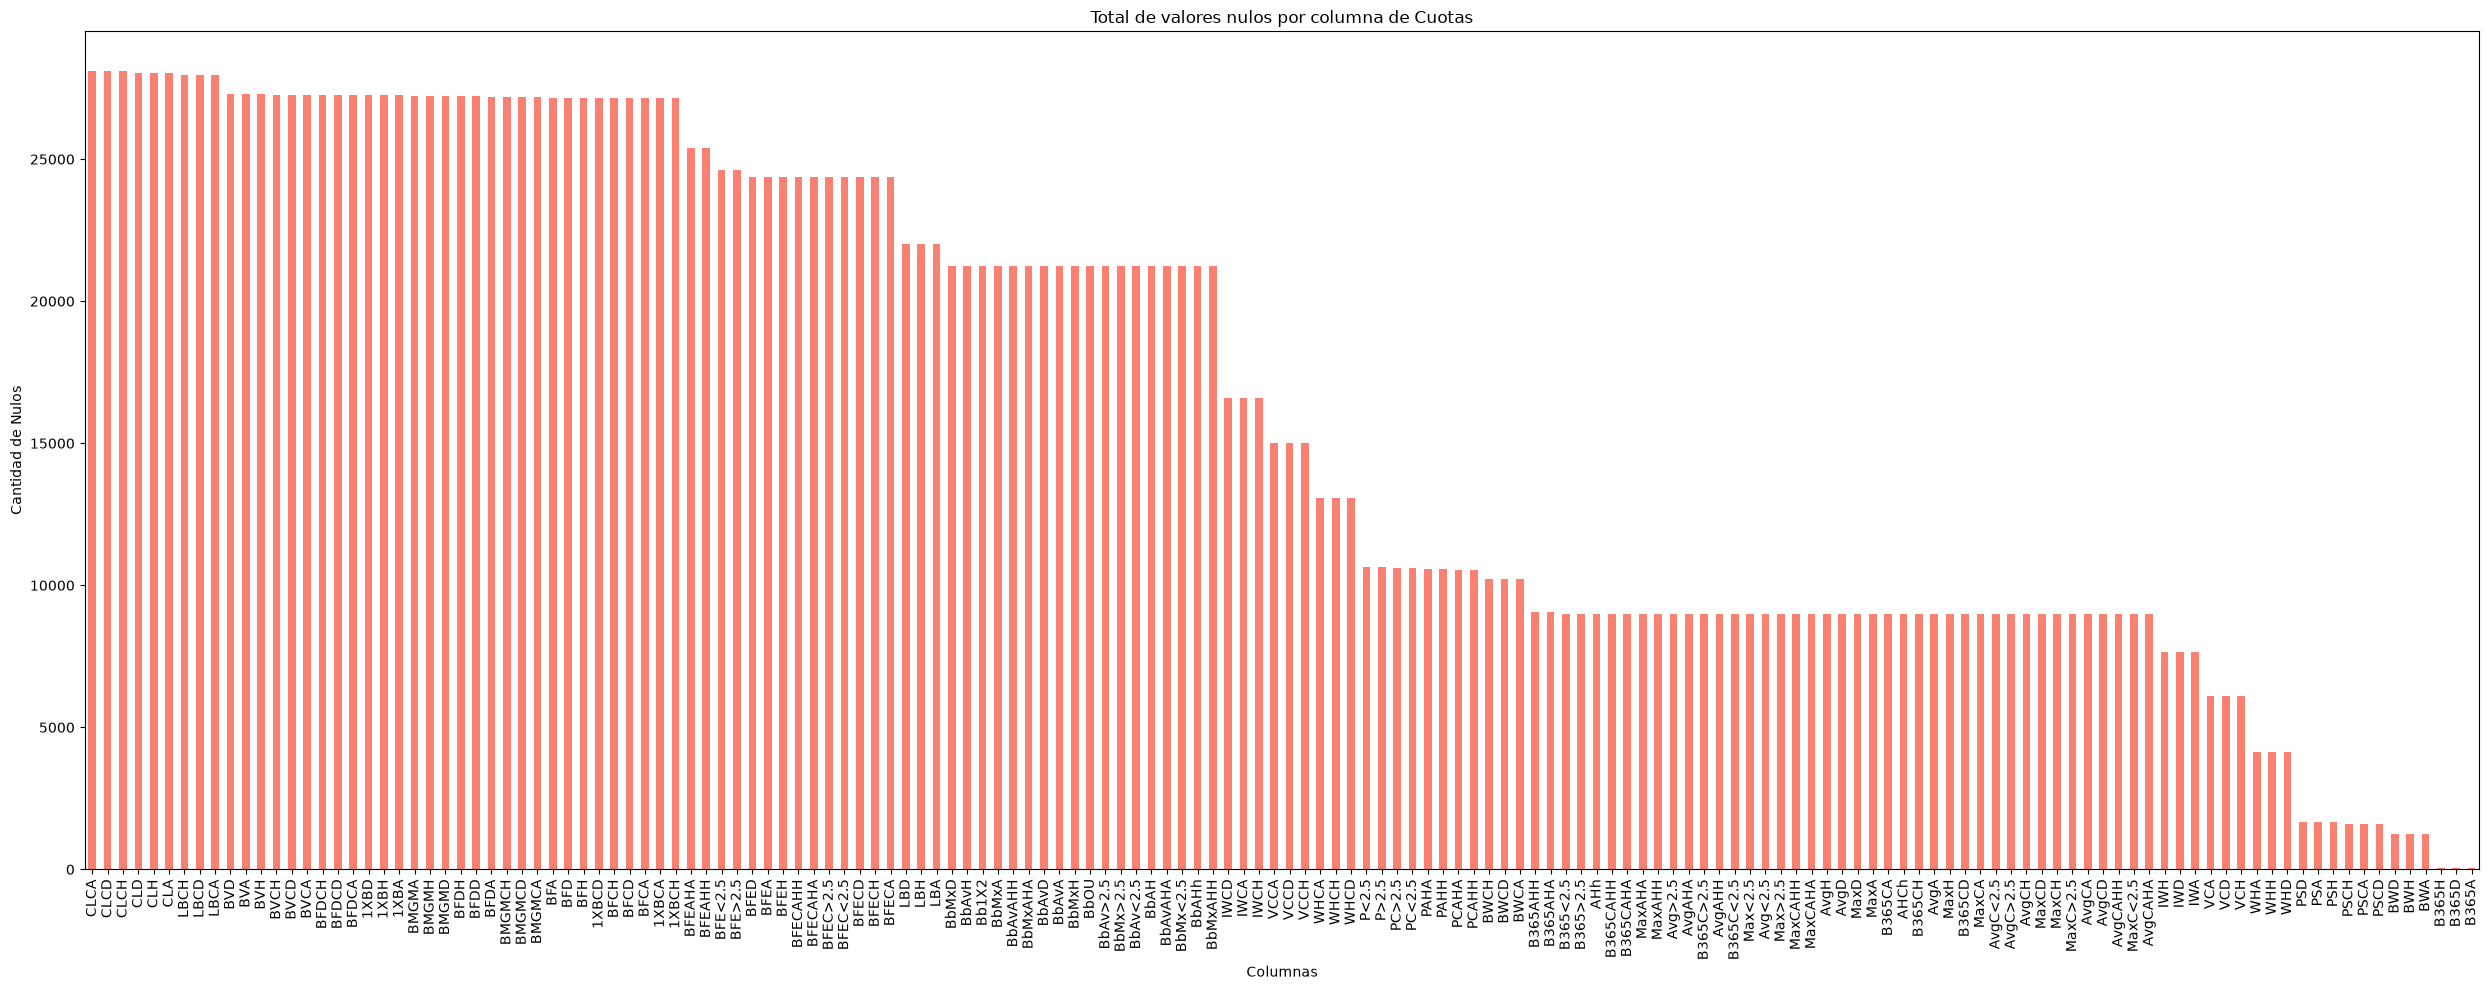
\includegraphics[width=\columnwidth]{figures/eda_nulos_cuotas.png}
\caption{Porcentaje de valores nulos por columna de cuotas. La banda superior ($> 40\%$) se descartó, la intermedia ($20$--$40\%$) se preservó como bandera de ausencia y el resto se imputó con KNN.}
\label{fig:nulos}
\end{figure}

Las columnas de cuota descartadas ( $> 40\%$  de nulos) corresponden a casas secundarias (Ladbrokes, Interwetten, Betfair, BetMGM, BetVictor, Colossus); las columnas entre 20\% y 40\% se convirtieron en banderas binarias \texttt{*\_Ausente}, capturando la señal de que el mercado suspendió o no ofreció el mercado (partidos oscuros, cuotas anómalas); las restantes con nulos positivos se imputaron con \texttt{KNNImputer} (k=5) previa estandarización, aprovechando la alta correlación entre casas.

\textbf{Valores faltantes en otras variables.} Además de las cuotas:
\begin{itemize}
    \item \texttt{Unnamed: 105}, \texttt{Unnamed: 119} y \texttt{Unnamed: 120}: 30{,}182 nulos (100\%), artefactos de concatenación eliminados.
    \item \texttt{HFKC}, \texttt{AFKC}: 29{,}704 nulos (98.4\%), eliminadas.
    \item \texttt{Referee}: 26{,}382 nulos (87.4\%), eliminada; era casi exclusivamente informativa para 2016/17--2018/19 y 2025/26.
    \item \texttt{Time}: 8{,}952 nulos (29.7\%), transformada a la numérica \texttt{Time\_hora}.
    \item \texttt{HTR}: 39 nulos, reconstruida a partir de \texttt{HTHG} y \texttt{HTAG} sin imputación estadística.
\end{itemize}
Tras la limpieza, el dataframe quedó sin valores nulos.

\textbf{Duplicados e integridad.} No se detectaron duplicados exactos de partidos. La clave compuesta \texttt{(Div, Season, Date, HomeTeam, AwayTeam)} identifica cada fila de forma única.

\textbf{Outliers.} Se aplicó la regla IQR, que considera atípicos los valores fuera de $[Q_1-1.5\,\mathrm{IQR},\,Q_3+1.5\,\mathrm{IQR}]$ (Figs.~\ref{fig:box} y~\ref{fig:hist}). Los extremos detectados en goles (hasta 10--13) y tiros (hasta 46) corresponden a partidos reales con marcadores inusuales; son legítimos y no se eliminan. Los outliers de cuotas medias de mercado (\texttt{AvgH} máx.~28.96, \texttt{AvgA} máx.~41.22, \texttt{AvgD} máx.~16.44) reflejan partidos muy desequilibrados, no errores de datos, y se conservan.

\begin{figure}[H]
\centering
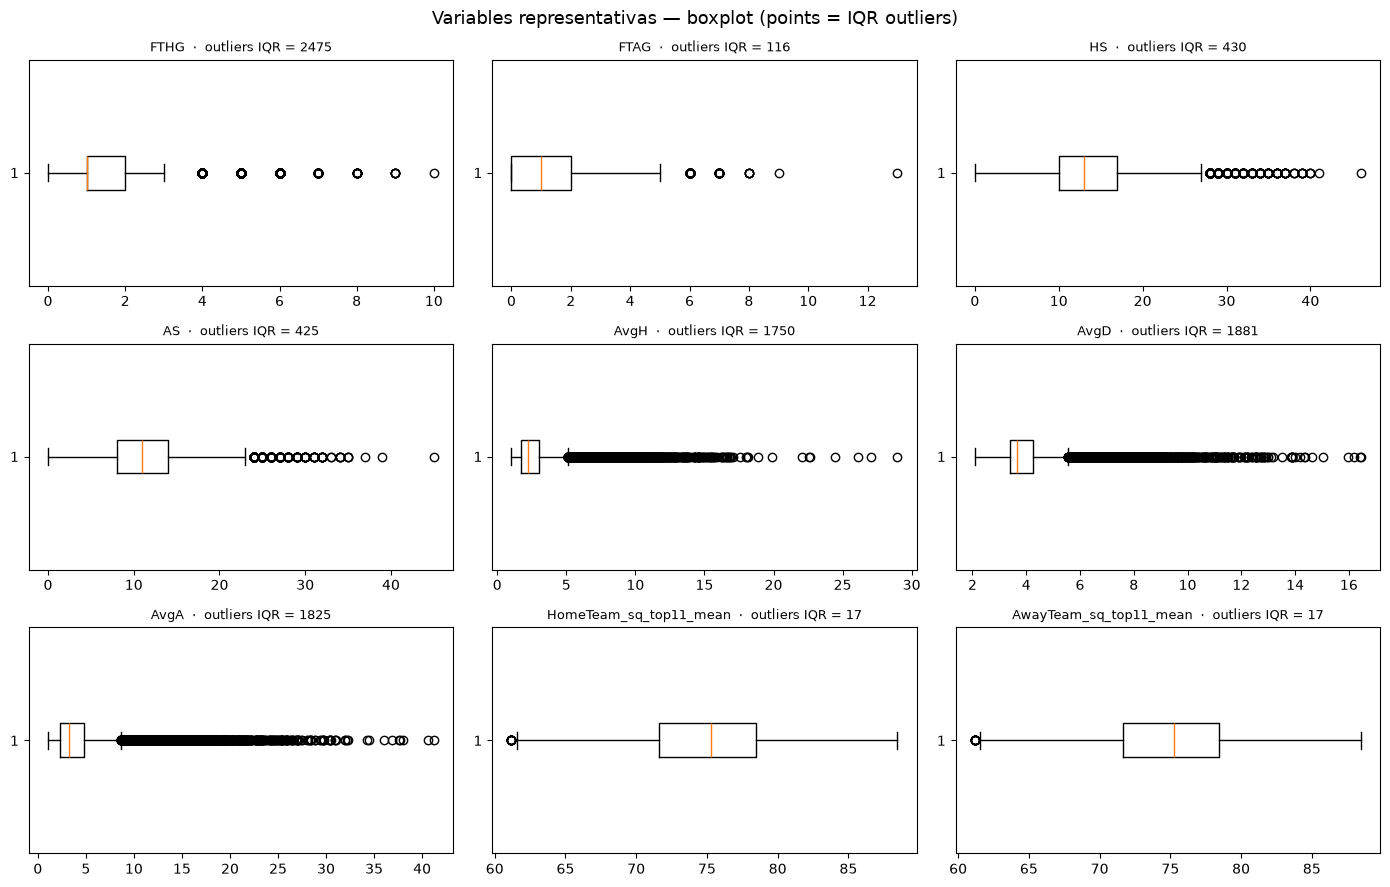
\includegraphics[width=\columnwidth]{figures/eda_boxplot_repr.png}
\caption{Boxplots con vallas de la regla IQR sobre variables representativas. Los extremos en goles y tiros son partidos reales, no errores.}
\label{fig:box}
\end{figure}

\begin{figure}[H]
\centering
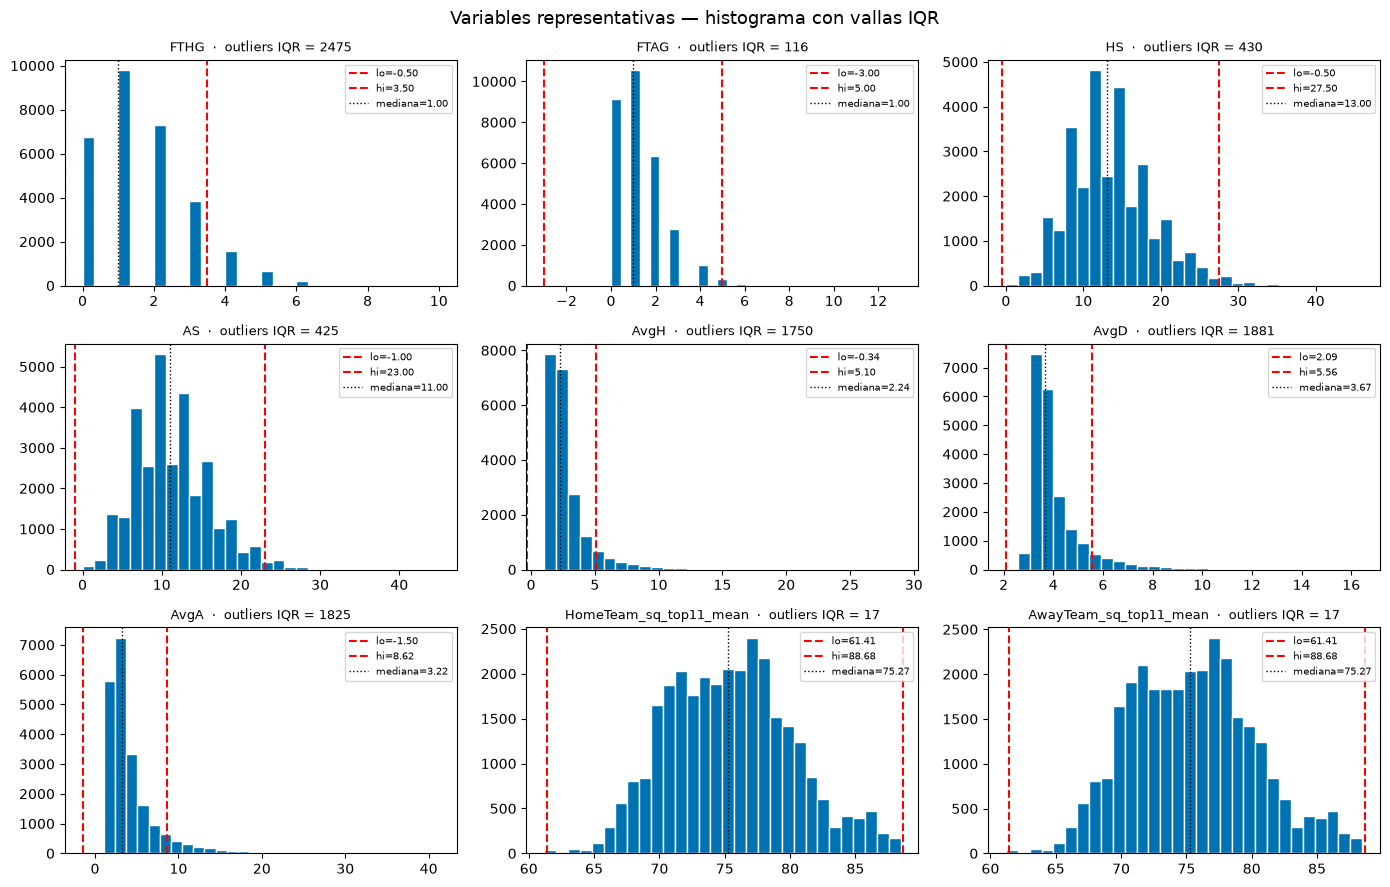
\includegraphics[width=\columnwidth]{figures/eda_hist_repr.png}
\caption{Histogramas con vallas IQR sobre las mismas variables representativas; la asimetría de goles y cuotas es consistente con la teoría.}
\label{fig:hist}
\end{figure}

\subsection{Análisis univariado}
Las variables numéricas siguen las distribuciones esperadas del fútbol (Tablas~\ref{tab:num1} y~\ref{tab:num2}). La ventaja de localía se refleja en que la media de goles del local supera en 0.31 a la del visitante (1.56 vs.\ 1.25), también visible en el medio tiempo (0.69 vs.\ 0.55).

\begin{table}[H]
\caption{Estadísticas descriptivas de las variables de fútbol}
\centering
\footnotesize
\begin{tabular}{lccccc}
\toprule
\textbf{Variable} & \textbf{Media} & \textbf{DE} & \textbf{Mín.} & \textbf{Mediana} & \textbf{Máx.} \\
\midrule
\texttt{FTHG} & 1.56 & 1.31 & 0 & 1 & 10 \\
\texttt{FTAG} & 1.25 & 1.18 & 0 & 1 & 13 \\
\texttt{HTHG} & 0.69 & 0.84 & 0 & 0 & 6 \\
\texttt{HTAG} & 0.55 & 0.76 & 0 & 0 & 7 \\
\texttt{HS}   & 13.52 & 5.37 & 0 & 13 & 46 \\
\texttt{AS}   & 11.13 & 4.79 & 0 & 11 & 45 \\
\texttt{HST}  & 4.89 & 2.61 & 0 & 5 & 20 \\
\texttt{AST}  & 4.03 & 2.37 & 0 & 4 & 23 \\
\texttt{HC}   & 5.41 & 2.97 & 0 & 5 & 26 \\
\texttt{AC}   & 4.45 & 2.64 & 0 & 4 & 19 \\
\texttt{HF}   & 12.34 & 4.10 & 0 & 12 & 33 \\
\texttt{AF}   & 12.55 & 4.12 & 0 & 12 & 34 \\
\texttt{HY}   & 1.94 & 1.39 & 0 & 2 & 10 \\
\texttt{AY}   & 2.17 & 1.44 & 0 & 2 & 10 \\
\texttt{HR}   & 0.10 & 0.32 & 0 & 0 & 3 \\
\texttt{AR}   & 0.11 & 0.34 & 0 & 0 & 3 \\
\bottomrule
\end{tabular}
\label{tab:num1}
\end{table}

\begin{table}[H]
\caption{Estadísticas descriptivas de cuotas medias de mercado, hora y plantilla.}
\centering
\footnotesize
\resizebox{\columnwidth}{!}{%
\begin{tabular}{lccccc}
\toprule
\textbf{Variable} & \textbf{Media} & \textbf{DE} & \textbf{Mín.} & \textbf{Mediana} & \textbf{Máx.} \\
\midrule
\texttt{AvgH} & 2.76 & 1.84 & 1.03 & 2.24 & 28.96 \\
\texttt{AvgD} & 4.07 & 1.22 & 2.09 & 3.67 & 16.44 \\
\texttt{AvgA} & 4.29 & 3.50 & 1.06 & 3.22 & 41.22 \\
\texttt{B365H} & 2.77 & 1.95 & 1.02 & 2.20 & 26.00 \\
\texttt{Time\_hora} & 16.59 & 2.3 & 10 & 17 & 22 \\
\texttt{HomeTeam\_sq\_overall\_mean} & 70.36 & 3.85 & 58.92 & 70.33 & 82.58 \\
\texttt{HomeTeam\_sq\_overall\_max} & 78.86 & 5.18 & 63 & 79 & 94 \\
\texttt{HomeTeam\_sq\_top11\_mean} & 75.37 & 4.78 & 61.18 & 75.27 & 88.45 \\
\bottomrule
\end{tabular}%
} 
\label{tab:num2}
\end{table}


Las cuotas medias de mercado (\texttt{AvgH}, \texttt{AvgD}, \texttt{AvgA}) tienen distribución fuertemente asimétrica a la derecha (media $>$ mediana) con cola larga hacia cuotas altas; la masa central se concentra en cuotas de favorito (bajas). Estas medias del mercado 1X2 son prácticamente equivalentes a las cuotas de cierre de Pinnacle (el acierto del favorito difiere en menos de 1 punto porcentual, 53.9\% vs.\ 54.5\%) y se usan como referencia del mercado por su mayor cobertura de datos. Presentan un 29.8\% de valores faltantes, por lo que en el EDA se analizan desde el dataset crudo y en el \textit{pipeline} de features se imputan con KNN. Las features de \textit{squad quality} tienen rangos acotados y esperados: \texttt{overall\_mean} entre 58.92 y 82.58 (media 70.41), \texttt{overall\_max} entre 63 y 94, y \texttt{top11\_mean} entre 61.18 y 88.45 (media 75.44), con desviaciones que distinguen clubes de élite del resto. La hora de inicio (\texttt{Time\_hora}) se concentra entre las 14:00 y las 19:00 (media 16.5).

Las variables categóricas presentan la cardinalidad de la Tabla~\ref{tab:cat}. \texttt{Season} es numérica con 10 valores (una por temporada). La alta frecuencia de nulos en \texttt{Referee} y \texttt{Time} se explicó en la Sección~\ref{sec:calidad}.

\begin{table}[H]
\caption{Cardinalidad, moda y nulos de las variables categóricas.}
\centering
\footnotesize
\begin{tabular}{lcccr}
\toprule
\textbf{Variable} & \textbf{Únicos} & \textbf{Moda} & \textbf{Frec. moda} & \textbf{Nulos} \\
\midrule
\texttt{Div}      & 9     & \texttt{E0}       & 3{,}800  & 0 \\
\texttt{Date}     & 2{,}152 & 22/12/2018      & 53      & 0 \\
\texttt{HomeTeam} & 280   & Crystal Palace   & 190     & 0 \\
\texttt{AwayTeam} & 280   & Tottenham        & 190     & 0 \\
\texttt{FTR}      & 3     & $H$              & 13{,}371 & 0 \\
\texttt{HTR}      & 3     & $D$              & 12{,}140 & 39 \\
\texttt{Referee}  & 50    & A Taylor         & 295     & 26{,}382 \\
\texttt{Time}     & 47    & 20:00            & 2{,}033  & 8{,}952 \\
\bottomrule
\end{tabular}
\label{tab:cat}
\end{table}

\subsection{Análisis bivariado}
Estudiamos cómo las cuotas y la calidad de plantilla se relacionan con el resultado real \texttt{FTR}: se identifica la señal que aprovechará el modelo y se motiva el orden de importancia de las \textit{features}.

\textbf{Relación entre cuotas y resultado.} Las cuotas medias de mercado (\texttt{AvgH}, \texttt{AvgD}, \texttt{AvgA}) son las variables más informativas y anticipan con alta precisión la probabilidad del resultado (Fig.~\ref{fig:cuotas}). Son prácticamente equivalentes a las cuotas de cierre de Pinnacle: el acierto del favorito difiere en menos de 1 punto porcentual (53.9\% vs.\ 54.5\%) y la información mutua con \texttt{FTR} es casi idéntica ($\approx$0.11 en las clases $H$ y $A$). Se usa \texttt{Avg} como representación del mercado por su mayor cobertura y simplicidad. Esto es consistente con la literatura \cite{knoll2020} y motiva su uso como \textit{baseline} del mercado.

\begin{figure}[H]
\centering
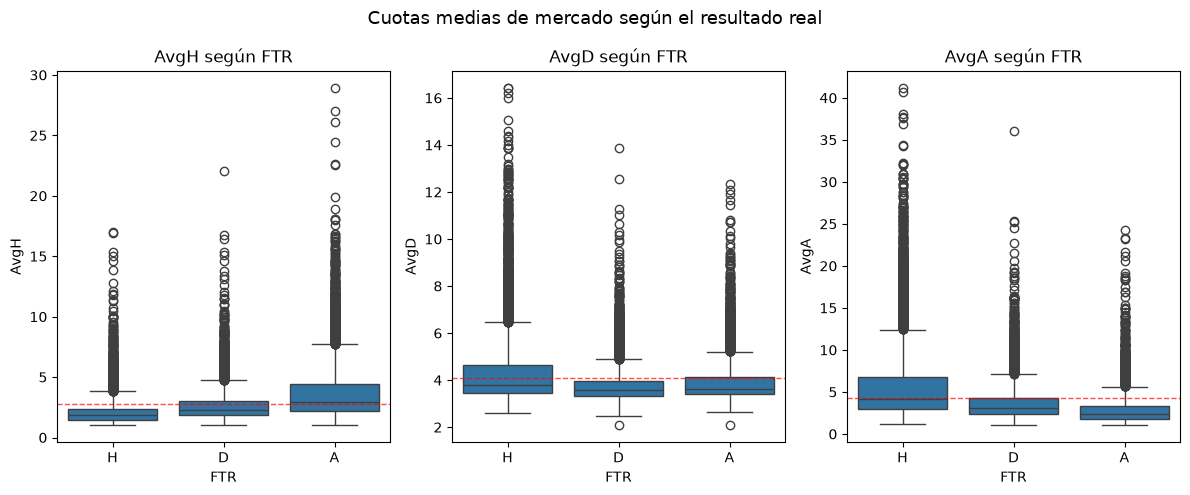
\includegraphics[width=\columnwidth]{figures/eda_cuotas_vs_ftr.png}
\caption{Cuotas medias de mercado 1X2 (\texttt{AvgH}, \texttt{AvgD}, \texttt{AvgA}) según el resultado real \texttt{FTR}. La cuota del local es menor en victorias locales, y las cuotas altas se asocian a empates/derrotas.}
\label{fig:cuotas}
\end{figure}

\textbf{Relación entre plantilla y resultado.} La diferencia de calidad entre onces (\texttt{HomeTeam\_sq\_top11\_mean} $-$ \texttt{AwayTeam\_sq\_top11\_mean}) correlaciona positivamente con la probabilidad de victoria local, aunque con magnitud menor que las cuotas (Fig.~\ref{fig:squad}). Su valor es complementario, sobre todo en las primeras jornadas cuando las estadísticas de forma son escasas.

\begin{figure}[H]
\centering
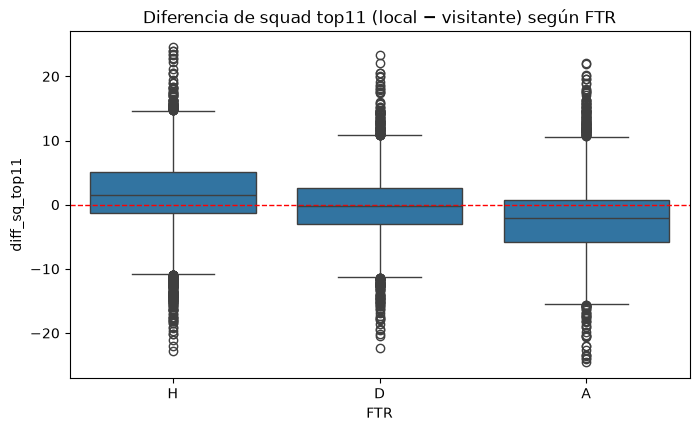
\includegraphics[width=\columnwidth]{figures/eda_squad_vs_ftr.png}
\caption{Diferencia de calidad de once según el resultado \texttt{FTR}: a mayor ventaja de plantilla, mayor proporción de victorias locales.}
\label{fig:squad}
\end{figure}

\subsection{Análisis multivariado}
En este apartado se interpreta cada gráfico multivariado: qué representa y qué información se extrae para el diseño de \textit{features}.

\textbf{Matriz de correlación (Fig.~\ref{fig:corr}).} El mapa de color muestra la correlación de Pearson entre todas las variables numéricas y el detalle anotado se restringe a las variables clave (goles, tiros, cuotas medias y \textit{squad}). Se confirma \textbf{multicolinealidad}: las cuotas del mismo mercado correlacionan con $|r|>0.9$ en la mayoría de pares, es decir, aportan información redundante. Esto justifica la imputación con KNN y motiva conservar una única referencia de mercado (\texttt{AvgH}/\texttt{AvgD}/\texttt{AvgA}) junto con las banderas \texttt{*\_Ausente} como representación compacta. Goles y tiros correlacionan positivamente ($r\approx0.6$--$0.7$) y la \textit{squad} correlaciona poco con las cuotas, lo que la convierte en señal complementaria.

\begin{figure}[H]
\centering
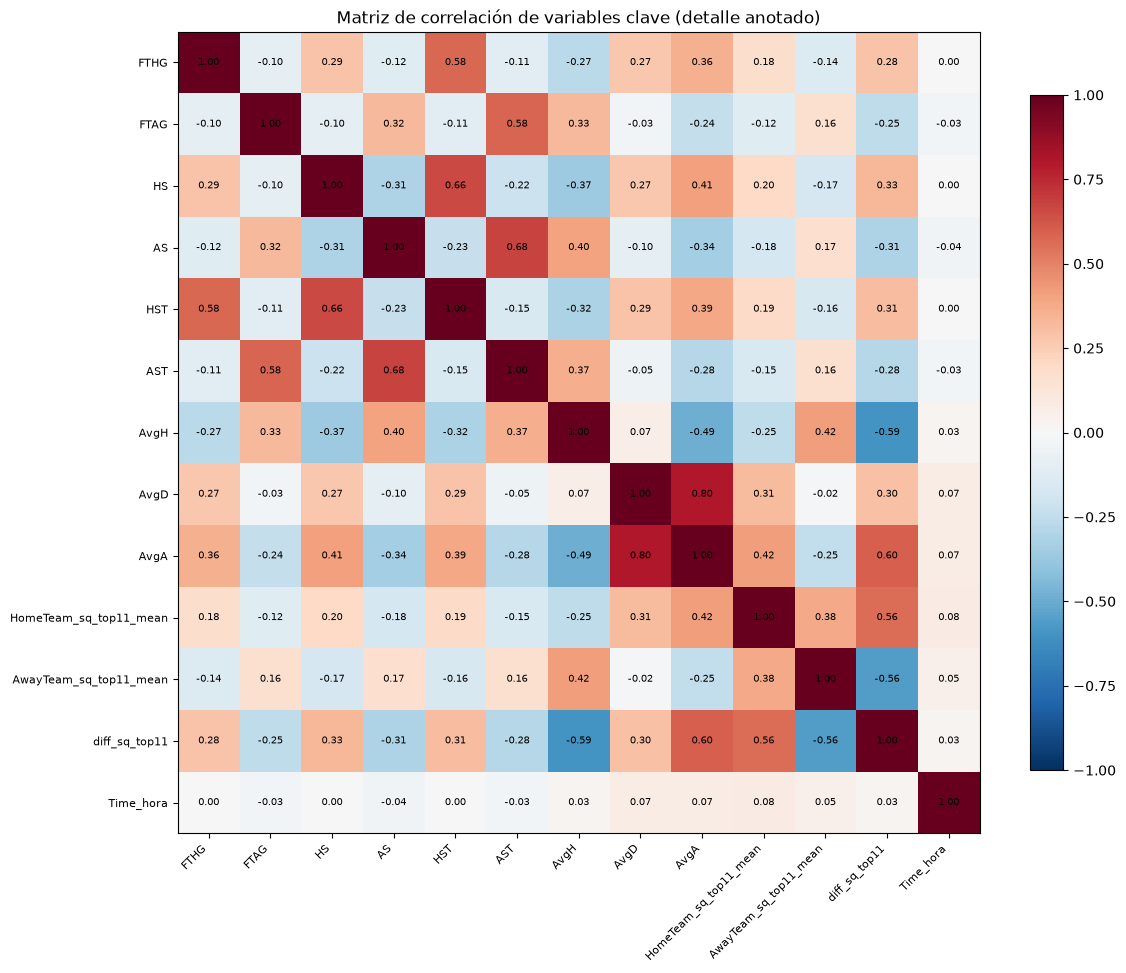
\includegraphics[width=\columnwidth]{figures/eda_corr_detalle.png}
\caption{Detalle de la matriz de correlación entre variables clave de cuotas medias, plantilla y estadísticas. Las cuotas del mismo mercado tienen $|r|>0.9$.}
\label{fig:corr}
\end{figure}

\textbf{\textit{Scatter matrix} o \textit{pairplot} (Fig.~\ref{fig:pair}).} Cada panel representa un par de variables clave (goles, cuotas medias, \textit{squad}) coloreado por \texttt{FTR} sobre una muestra de 5{,}000 partidos. Las tres clases se solapan sustancialmente (el fútbol es ruidoso), pero los pares de goles y de cuotas medias muestran la mejor separación parcial, mientras que la \textit{squad} (\texttt{diff\_sq\_top11}) aporta fronteras más difusas.

\begin{figure}[H]
\centering
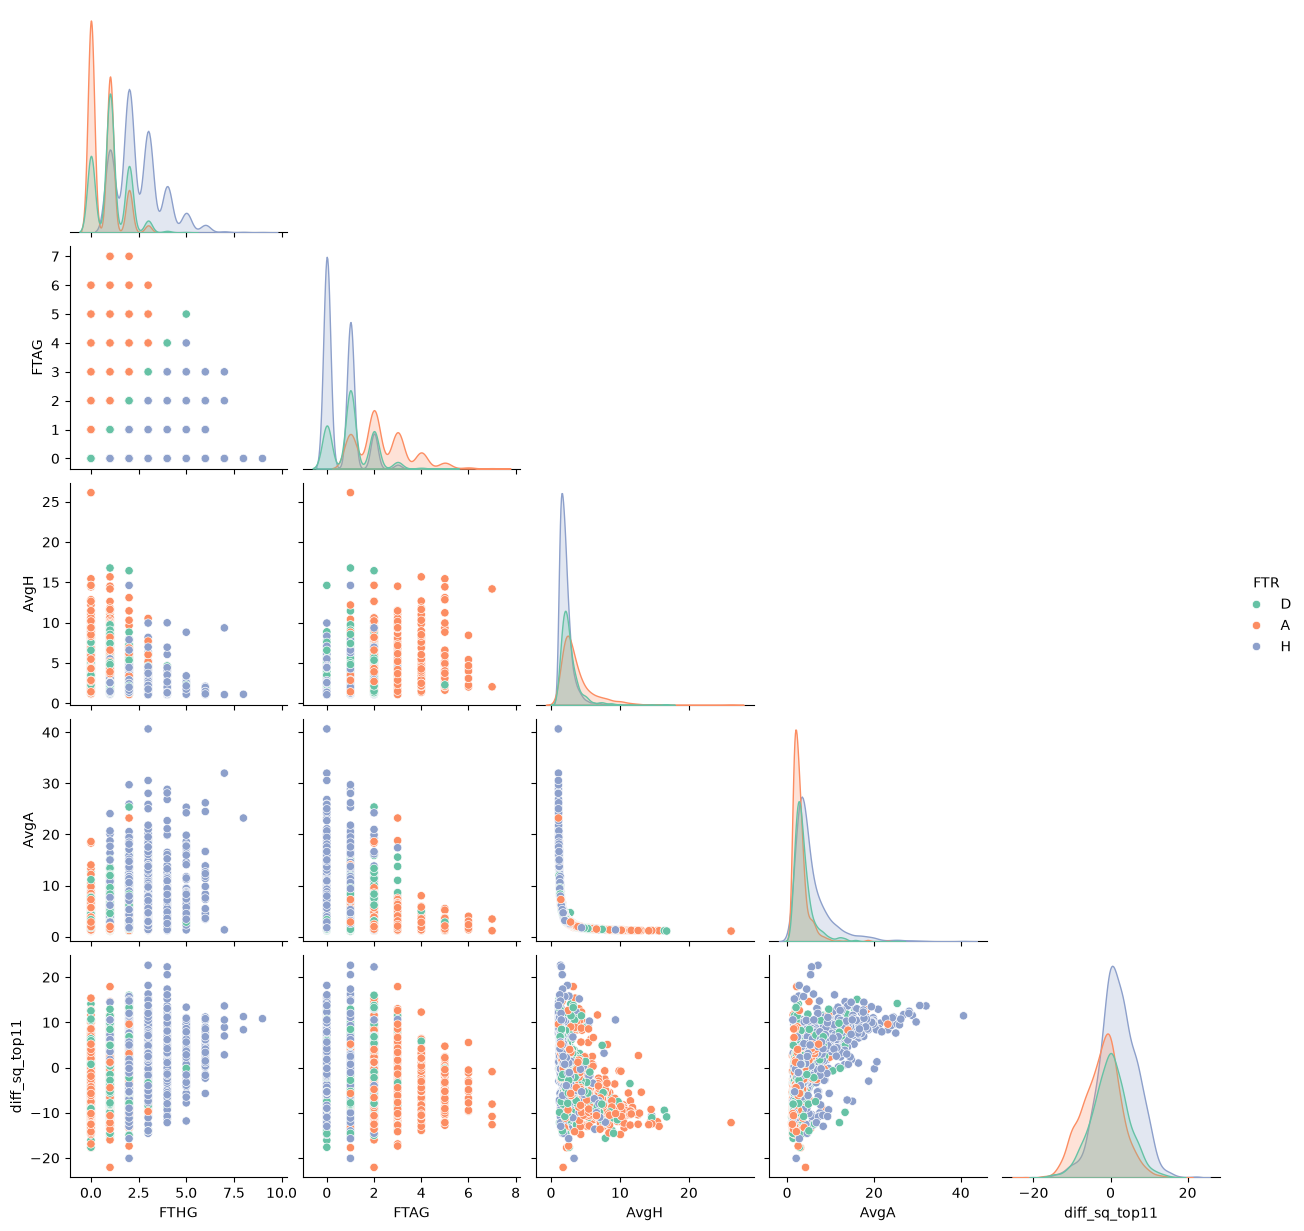
\includegraphics[width=\columnwidth]{figures/eda_pairplot.png}
\caption{\textit{Pairplot} de variables seleccionadas coloreado por \texttt{FTR}. Las cuotas medias de mercado separan mejor las clases que las estadísticas crudas.}
\label{fig:pair}
\end{figure}

\textbf{Análisis de componentes principales (Fig.~\ref{fig:pca}).} La PCA proyecta las cuotas medias de mercado (variables altamente correlacionadas) en dos componentes ortogonales. Los dos primeros componentes retienen prácticamente toda la varianza del mercado 1X2 (las cuotas son casi colineales): comprimir el mercado en pocas variables no pierde señal apreciable. No se observan \textit{clusters} separables: el extremo de PC1 (cuota de local muy baja, favorito claro) se concentra en victorias locales y la nube central corresponde a partidos equilibrados y empates, coherente con un problema de margen estrecho entre clases.

\begin{figure}[H]
\centering
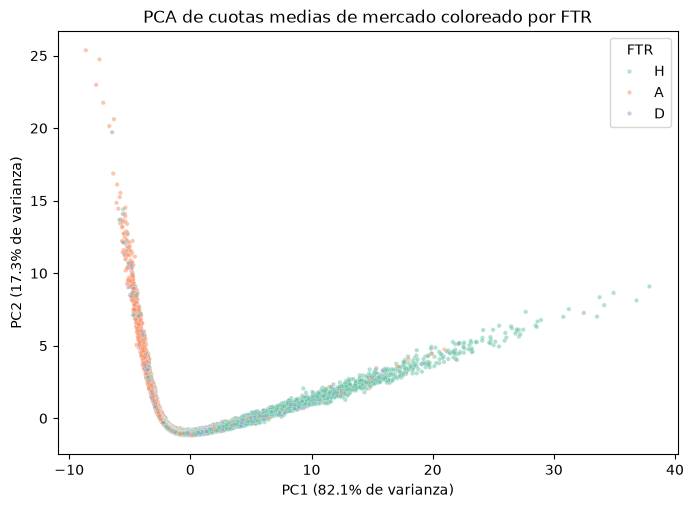
\includegraphics[width=\columnwidth]{figures/eda_pca.png}
\caption{Proyección PCA en 2 componentes de las cuotas medias de mercado. No hay \textit{clusters}, coherente con un problema de margen estrecho.}
\label{fig:pca}
\end{figure}

\subsection{Posibles sesgos y data leakage}
Este es probablemente el punto más crítico del análisis exploratorio:

\begin{itemize}
    \item \textbf{Data leakage por estadísticas post-partido.} \texttt{FTHG}, \texttt{FTAG}, \texttt{HS}, \texttt{AS}, \texttt{HST}, \texttt{AST}, \texttt{HC}, \texttt{AC}, \texttt{HF}, \texttt{AF}, \texttt{HY}, \texttt{AY}, \texttt{HR} y \texttt{AR} se conocen \textit{después} del partido. Usarlas directamente sería \textit{leakage} trivial. La solución es transformarlas en medias \textit{rolling} de los últimos $N$ partidos por equipo, respetando el orden temporal.
    \item \textbf{\textit{Data leakage} por \textit{look-ahead}.} Cualquier agregación (medias por equipo, fuerza de plantilla) debe calcularse con información estrictamente anterior a la fecha del partido. El \textit{split} train/test será cronológico, nunca aleatorio.
    \item \textbf{Sesgo de plantilla por temporada.} Los ratings EA se publican al inicio de la temporada; el snapshot de una temporada no debe usarse para predecir la anterior. El pipeline ya usa un solo snapshot por temporada.
    \item \textbf{Sesgo de cobertura.} La Premier League (E0) aporta 3{,}800 partidos, mientras que la Pro League (B1) aporta 2{,}805; ligas con menos historia pueden quedar sub-representadas. Se mitiga con validación por liga y temporada.
    \item \textbf{Sesgo de cuotas.} Excluir cuotas de casas con muchos nulos y usar banderas de ausencia puede introducir sesgo si el patrón de ausencia no es aleatorio; precisamente por ello la ausencia se preserva como bandera binaria.
    \item \textbf{Sesgo de privacidad.} No hay PII en el dataset: los identificadores de jugadores ya vienen seudonimizados por las fuentes originales.
\end{itemize}

\subsection{Hallazgos principales del EDA}
Sintetizamos el EDA en seis hallazgos accionables para el modelado:

\begin{enumerate}
    \item El dataset consolidado contiene \textbf{30{,}182 partidos y 219 columnas útiles}, con cobertura temporal y de liga suficiente para modelar.
    \item La variable objetivo está \textbf{levemente desbalanceada} (H = 44.3\%, A = 30.9\%, D = 24.8\%); se usará como \textit{prior} y no se rebalanceará.
    \item La \textbf{calidad de los datos} es buena tras un proceso explícito de limpieza: se eliminaron 83 columnas de cuotas de baja cobertura, se crearon 58 banderas de ausencia y se imputaron con KNN 15 columnas restantes, quedando el dataset sin nulos.
    \item Las features más informativas pre-partido son las \textbf{cuotas medias de mercado} (representadas por \texttt{AvgH}/\texttt{AvgD}/\texttt{AvgA}, prácticamente equivalentes a las de cierre de Pinnacle), seguidas por las features de \textbf{squad quality} (\texttt{overall\_mean}, \texttt{top11\_mean} y \texttt{top3} por línea).
    \item El mayor riesgo metodológico es el \textbf{\textit{data leakage} temporal}: las estadísticas de partido deben desfasarse y el \textit{split} debe ser cronológico.
    \item Existen \textbf{outliers legítimos} en goles y tiros que no se eliminan; los outliers de cuotas son informativos y se conservan.
\end{enumerate}

\subsection{Trabajo futuro derivado del EDA}
Con base en los hallazgos, se propone el siguiente plan de modelado:
\begin{enumerate}
    \item \textbf{Preprocesamiento temporal}: eliminar columnas post-partido, construir features \textit{rolling} (últimos 5 partidos) por equipo, y limpiar el dataset.
    \item \textbf{Ingeniería de features}: agregar features de \textit{squad quality} (ya disponibles) y relativizar por liga/temporada con z-scores (\texttt{*\_sq\_*\_z}) para corregir la inflación de ratings de EA a lo largo del tiempo.
    \item \textbf{Selección de features}: aplicar \texttt{mutual\_info\_classif} y comparar contra entrenar sin selección.
    \item \textbf{Modelos}: \textit{baseline} mayoritario, regresión logística, Random Forest, XGBoost y MLP; ensemble por promedio de probabilidades.
    \item \textbf{Evaluación}: \textit{log loss}, Brier, accuracy y $F_1$ macro; diagramas de calibración; validación por temporada.
    \item \textbf{Backtest de \textit{value bets}}: comparar probabilidad estimada contra cuotas de cierre y calcular ROI por apuesta con umbral de valor.
\end{enumerate}

\begin{thebibliography}{10}
\bibitem{tammouch2024} Y. Tammouch, A. Elouafi, and I. Essadik, ``Betting on Machine Learning: Extracting Patterns from Football's Anarchic Odds,'' 2024.
\bibitem{knoll2020} J. Knoll and J. Stübinger, ``Machine-Learning-Based Statistical Arbitrage Football Betting,'' \textit{Applied Sciences}, vol. 10, no. 19, 2020.
\bibitem{dixon1997} M. J. Dixon and S. G. Coles, ``Modelling Association Football Scores and Inefficiencies in the Football Betting Market,'' \textit{Applied Statistics}, vol. 46, no. 2, pp. 265--280, 1997.
\bibitem{karlis2003} D. Karlis and I. Ntzoufras, ``Analysis of sports data using bivariate Poisson models,'' \textit{The Statistician}, vol. 52, no. 3, pp. 381--393, 2003.
\bibitem{footballdata} football-data.co.uk, ``Football Data Historical Results and Betting Odds,'' \url{https://football-data.co.uk/data.php}, 2025.
\bibitem{kagglefifa} Kaggle, ``FIFA / EA Sports FC Player Ratings Datasets,'' \url{https://www.kaggle.com/datasets/}, 2025.
\end{thebibliography}

\end{document}